% ME3050 -  Dynamics Modeling and Controls - Tennessee Technological University
% Tristan Hill - Spring 2020 - Summer 2020 - Spring 2022
% Dynamics Modeling and Controls
% Lecture Module - Alternate Model Forms  - Topic 2  - Transfer Functions and Block Diagrams

% Document settings

\documentclass{beamer}                  % for presentation ?
%\documentclass[handout]{beamer}  % for handout ?

\usepackage{/home/thill/Documents/lectures/dmc_lectures/dmc_lectures}

\newcommand{\MNUM}{2\hspace{2mm}} % Module number
\newcommand{\TNUM}{1\hspace{2mm}} % Topic number 
\newcommand{\moduletitle}{Alternate Model Forms} % Titles and Stuff
\newcommand{\topictitle}{Tranfer Functions and Block Diagrams} 

\newcommand{\sectiontitleI}{Free and Forced Response} % More Titles and Stuff
\newcommand{\sectiontitleII}{Transfer Function Concept}
\newcommand{\sectiontitleIII}{Block Diagram - Basic Shapes}
\newcommand{\sectiontitleIV}{Block Diagrams - Mathematical Operations}
\newcommand{\sectiontitleV}{Block Diagram - Feedback Loops}

\author{ME3050 - Dynamic Modeling and Controls}
\title{Lecture Module - \moduletitle}
\date{Mechanical Engineering\vspc Tennessee Technological University}

\begin{document}
	
	\lstset{language=MATLAB,basicstyle=\ttfamily\small,showstringspaces=false}
	
	\frame{\titlepage \center\begin{framed}\Large \textbf{Topic \TNUM - \topictitle}\end{framed} \vspace{5mm}}
	
	% Section 0 - Outline
\frame{
	
	\large \textbf{\moduletitle} \vspace{3mm}\\
	
	\begin{itemize}
	
		\item \hyperlink{sectionI}{\sectiontitleI} \vspc % Section I
		\item \hyperlink{sectionII}{\sectiontitleII} \vspc % Section II
		\item \hyperlink{sectionIII}{\sectiontitleIII} \vspc %Section III
		\item \hyperlink{sectionIV}{\sectiontitleIV} \vspc %Section IV	
		\item \hyperlink{sectionV}{\sectiontitleV} \vspc %Section V
	
	\end{itemize}

}

% Section I
\section{\sectiontitleI}

	% Section I - Frame I
	\begin{frame}[label=sectionI] \small
		\frametitle{\sectiontitleI}

		\btVFill
		\tiny{System Dynamics, Palm, 4$^{th}$}	

	\end{frame}

	%\section{\sectiontitleII}	
	
	% Section I - Frame II
	\begin{frame}[label=sectionI] \small
		\frametitle{\sectiontitleI}
		%\bigskip
		

		\btVFill
		\tiny{System Dynamics, Palm, 4$^{th}$}		
		
	\end{frame}

% Section II
\section{\sectiontitleII}

	% Section II - Frame I
	\begin{frame}[label=sectionII,containsverbatim] \small
			\frametitle{\sectiontitleII}

			\vspace{3mm}
		The transfer function is a way of describing a system that can be used to analyze the system response to an external input with the assumption of zero intial conditions.  

			
		\[ T(s)=\frac{X(s)}{F(s)} \]
		\vspace{10mm}
		Does this look familiar? How can we find the transfer function?		

	\end{frame}

	%Section II - Frame II
	\begin{frame} \small
		\frametitle{\sectiontitleII}
			
	\end{frame}	

% Section III
\section{\sectiontitleIII}

	% Section III - Frame I
	\begin{frame}[label=sectionIII] \small
		\frametitle{\sectiontitleIII}

		\vspace{3mm}	
		A block diagram is a visual representation of the transfer function concept. Here are the four basic symbols.

		\vspace{5mm}

		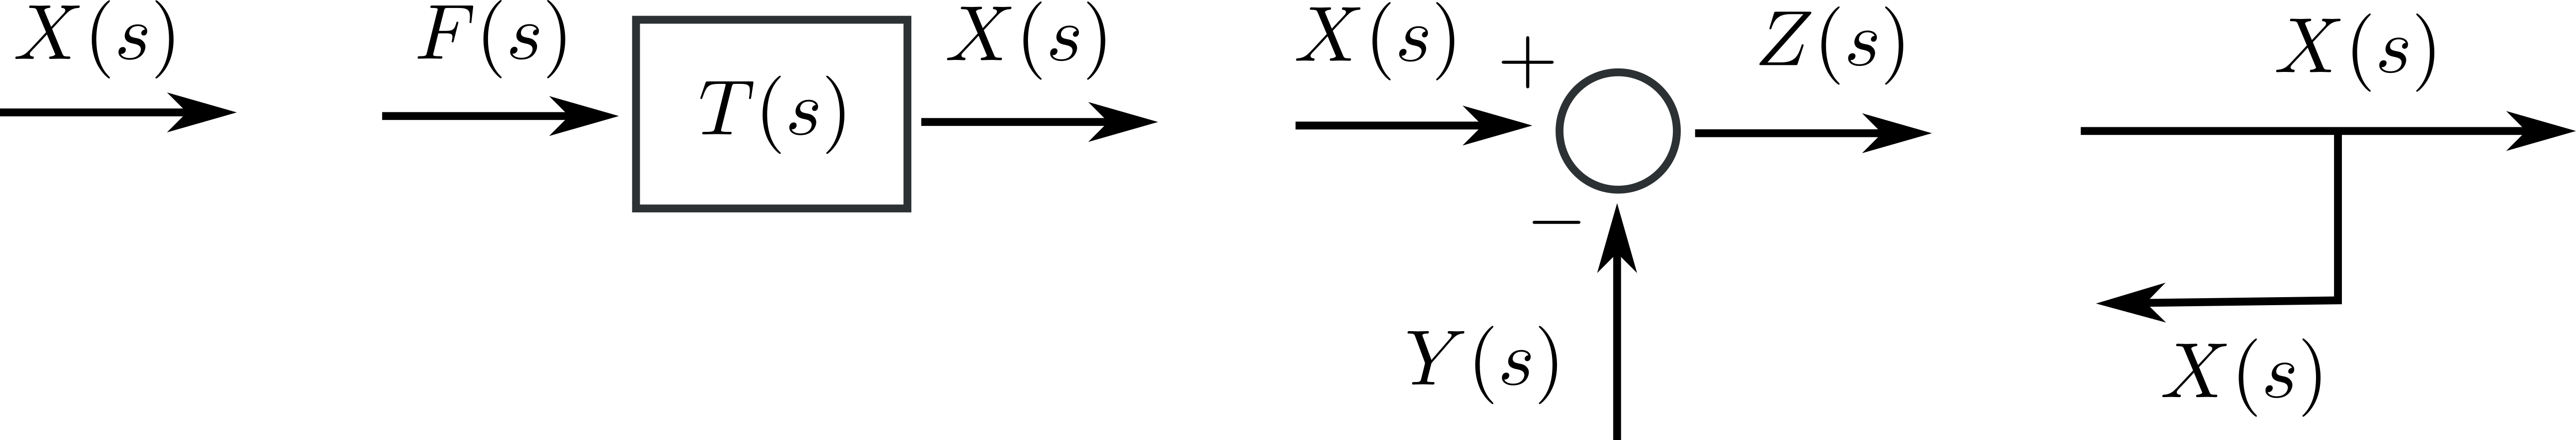
\includegraphics[scale=.04]{four_basic_symbols.png} \vspace{2mm}\\

	

		\btVFill

		\btVFill
	\end{frame}	
	
	%Section III - Frame II
	\begin{frame} \small
	

	\end{frame}	



% Section IV
\section{\sectiontitleIV}

	% Section IV - Frame I
	\begin{frame}[label=sectionIV] \small
		\frametitle{\sectiontitleIV}
		

		Mathematical operations can be represented as block diagrams. \vspace{2mm}\\

		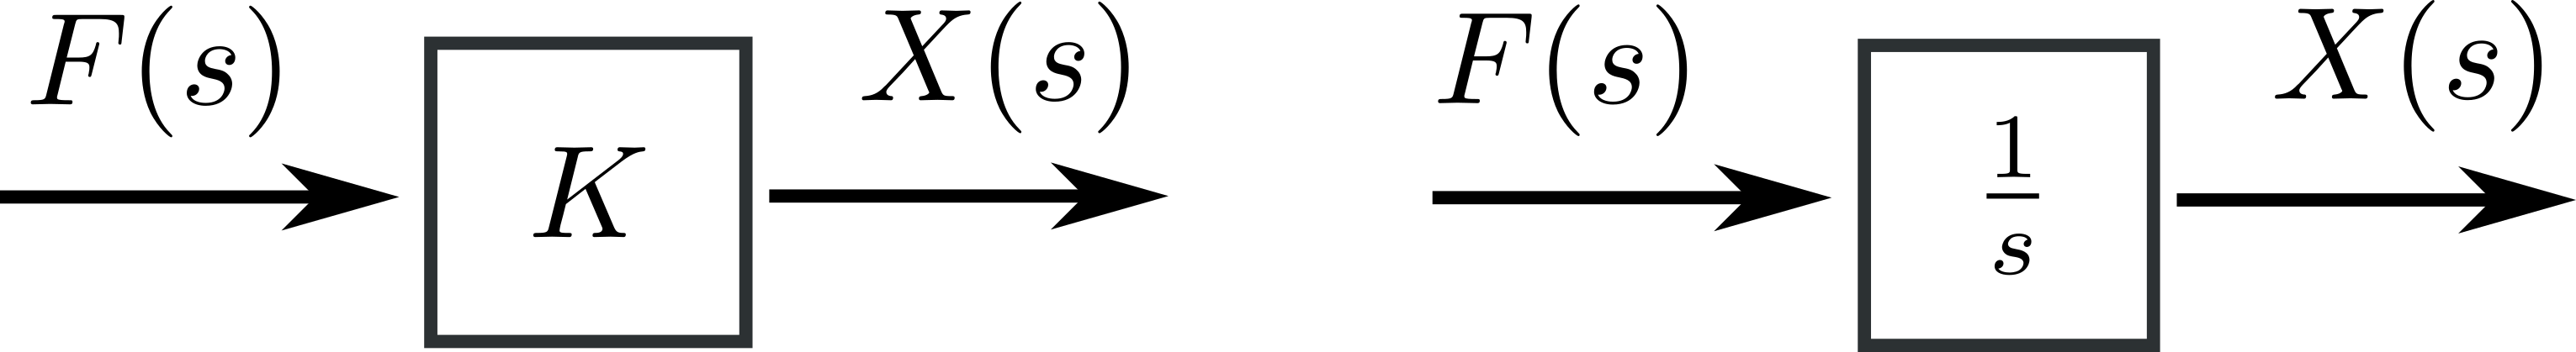
\includegraphics[scale=.04]{two_types_blocks.png}
	\end{frame}	

% Section V
\section{\sectiontitleV}

	% Section V - Frame I
	\begin{frame}[label=sectionV] \small
		\frametitle{\sectiontitleV}

		Block diagrams are used to represent feedback loops. \vspace{5mm} \\
		
		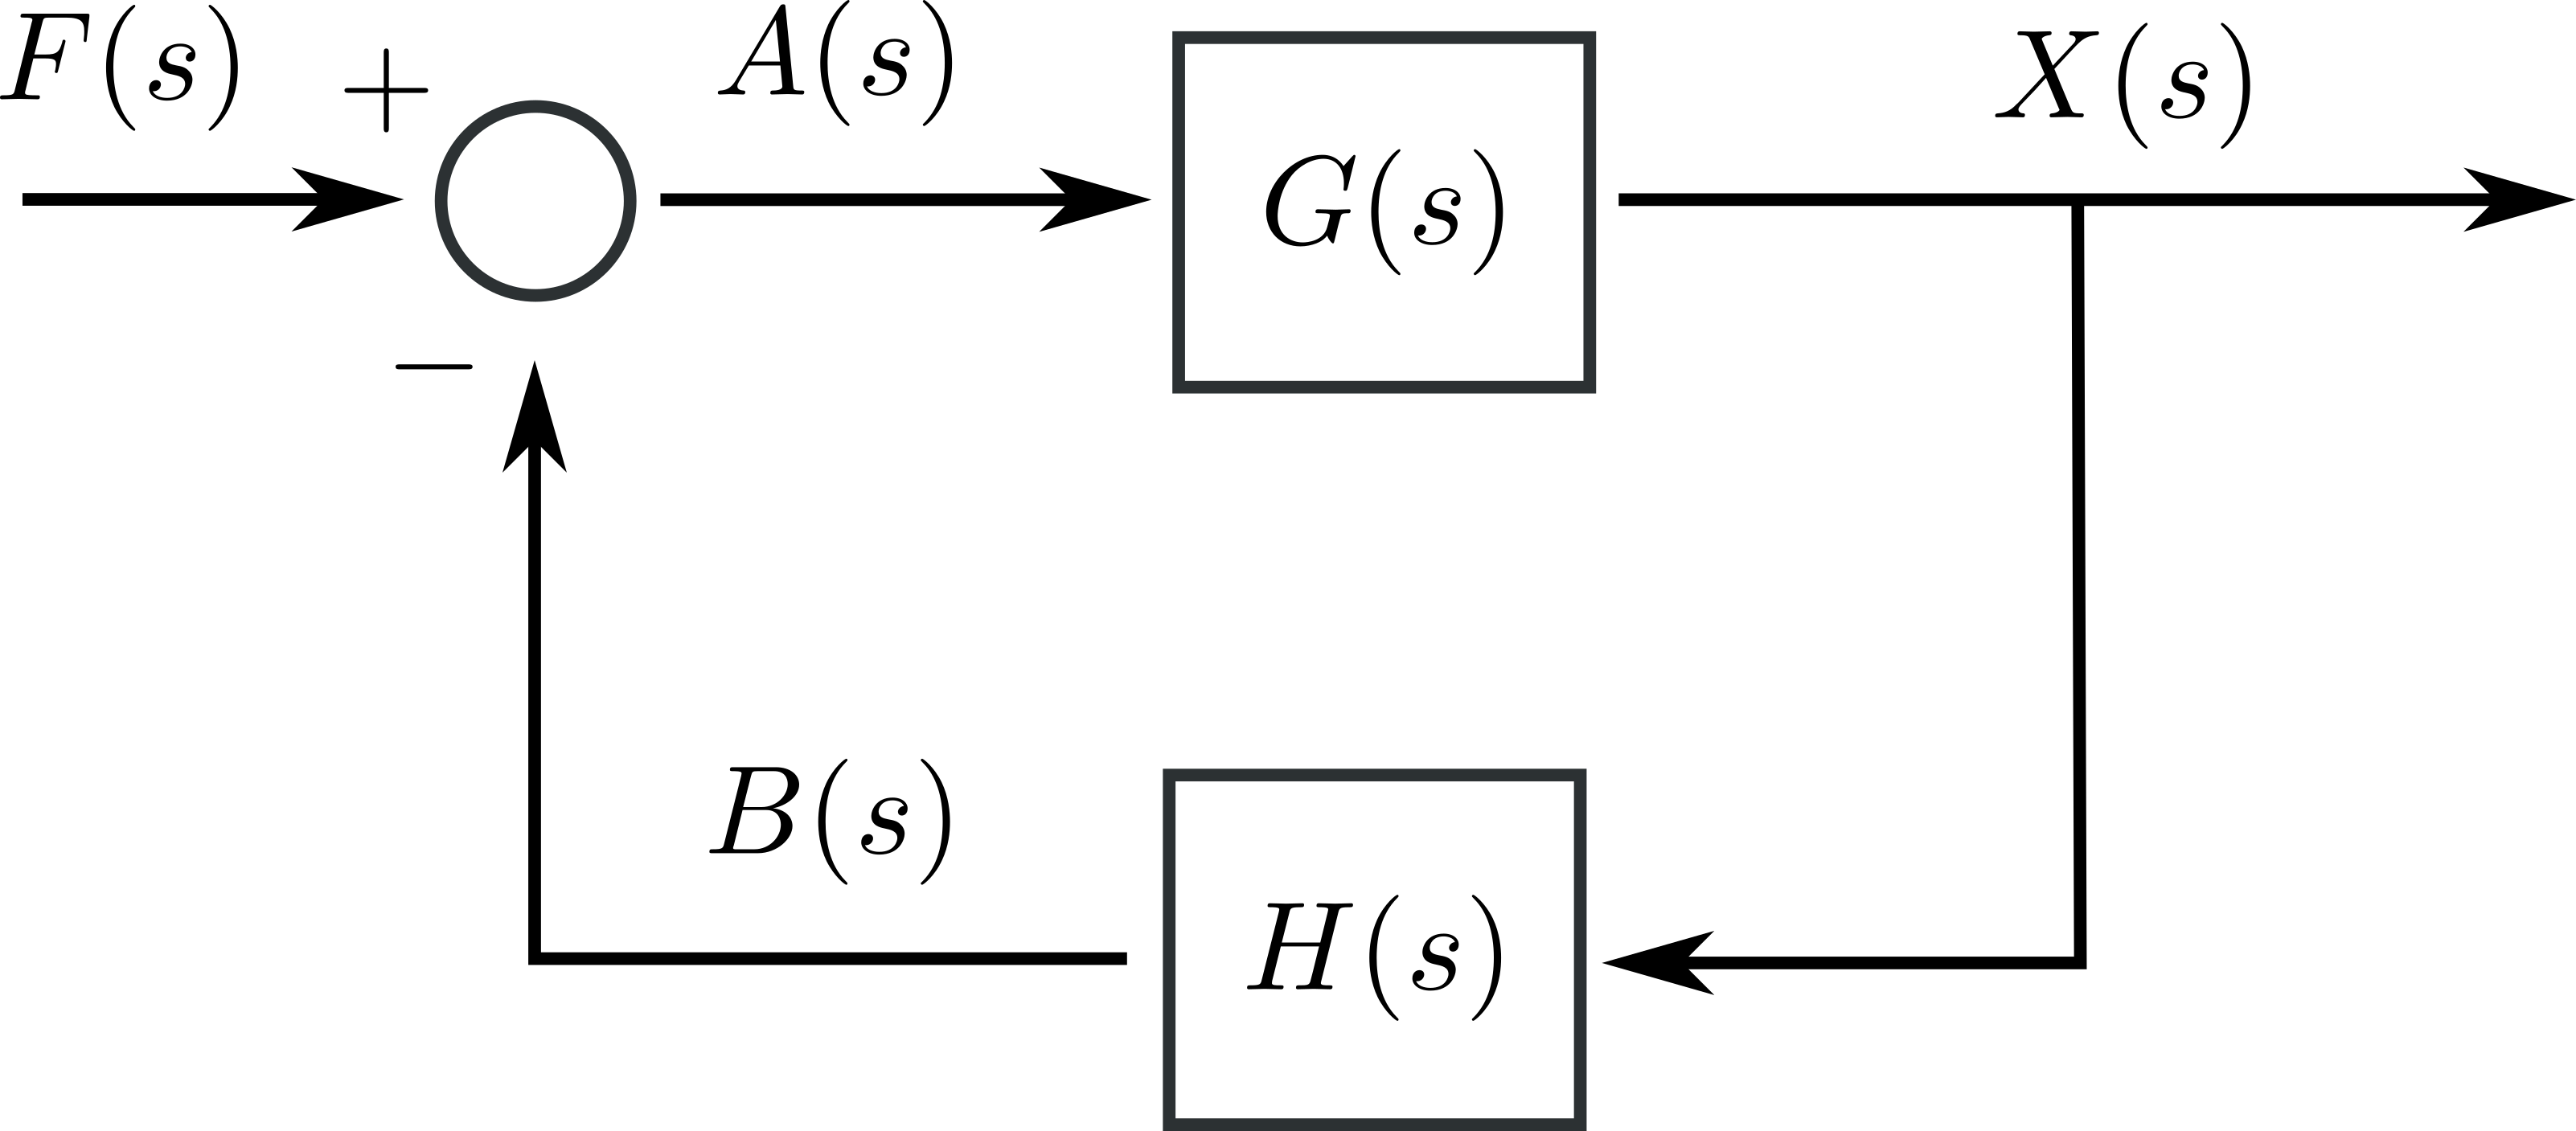
\includegraphics[scale=0.04]{generalized_feedback_loop.png} \vspace{5mm} \\

		 This block diagram can be simplified into a single equivilent block. Can you determine what that is?	

		\btVFill
		\tiny{Images: T.Hill - Original Images from System Dynamics, Palm, 4$^{th}$}

	\end{frame}	

\end{document}



